\part{Dokumentation}
\chapter{Einleitung}
Die vorliegende Dokumentation beschreibt den Programmablauf sowie die Klassenstruktur.
Bei der App handelt es sich um einen Taschenrechner, der komplexe Ausdrücke nach den gängigen Regeln berechnen kann und diese in einer ansehnlichen mathematischen Form (mathml) auf das Display ausgibt.
Ein solcher Ausdruck kann mit einer Grammatik beschrieben werden. 

Folgende erweiterte Backus-Naur-Form bildet die Grundlage für das vorliegende Programm:

\lstinputlisting{grammar_bnf.txt}
Die Grammatik gibt dabei an, wie der Syntaxbaum im Rechner aufgebaut wird.
Gleichzeitig wird damit die Bindungsstärke der Operatoren geregelt, 
nämlich von außen die Addition/Subtraktion (schwache Bindung) bis nach innen der Exponentialoperator (starke Bindung). 

\section{Umsetzung für iOs}
Normalerweise dient eine Grammatik dazu, Text von der Tastatur oder aus Textfiles zu parsen. Für den Taschenrechner auf iOs-Basis bringt dies aber Nachteile mit sich:
\begin{itemize}
	\item Es wird nur eine beschränkte Anzahl von Zeichen und Symbolen benötigt, 
		wobei die benötigten Symbole überwiegend mathematisch sind.
	\item Beim Navigieren über den Ausdruck (und Löschen von Elementen) gibt es Schwierigkeiten, 
		schließlich hat mein keinen Texteditor vor sich.
	\item Eine ``schöne'' mathematische Darstellung ist kaum möglich, es müsste eine Art Programmiersprachensyntax verwendet werden, oder die Ausgabe im getrennten Display erfolgen (Platzmangel)
	\item Es können durch falsche Eingaben viele Fehler auftreten $\rarr$ Benutzerunfreundliches debugging.
\end{itemize}
Stattdessen wird folgende Vorgehensweise forciert:
\begin{itemize}
	\item Die Symbole aus der Grammatik werden in eine Klassenstruktur umgewandelt.
	\item Der ``Objekt-Syntaxbaum'' baut sich dann praktisch selbst auf.
	\item Die ``Zeichen'' die hinzugefügt werden können, werden direkt als Methode an den Syntaxelementen definiert. Jedes Syntaxelement kann dann abhängig von seinem Kontext entscheiden, wie es auf die Eingabe reagieren soll.
	\item die Eingabemethoden werden dann über den ViewController mit Buttons in der View verknüpft.
	\item Jedes Element erzeugt seine Ausgabe selbst als mathml. Damit wird der Objektbaum in eine HTML/XML-Struktur transformiert.  Das damit aufgebaute HTML kann dann in einer UIWebView ausgegeben werden.
\end{itemize}
Dieses Vorgehen bietet folgende Vorteile:
\begin{itemize}
	\item Eingabefehler werden minimiert, da die (Syntax-) Elemente nur definierte Eingaben akzeptieren. Unpassendes kann einfach ignoriert werden.
	\item Eingabe erfolgt nur über Buttons, die Ausgabe ``live'' über HTML.
	\item Änderungen und die Navigation kann direkt über die Syntaxbaumelemente erfolgen, statt über einzelne Zeichen.
\end{itemize}

\chapter{Programmablauf}

\begin{figure}[H]
	\centering
	\label{dia:sq:trigger}
	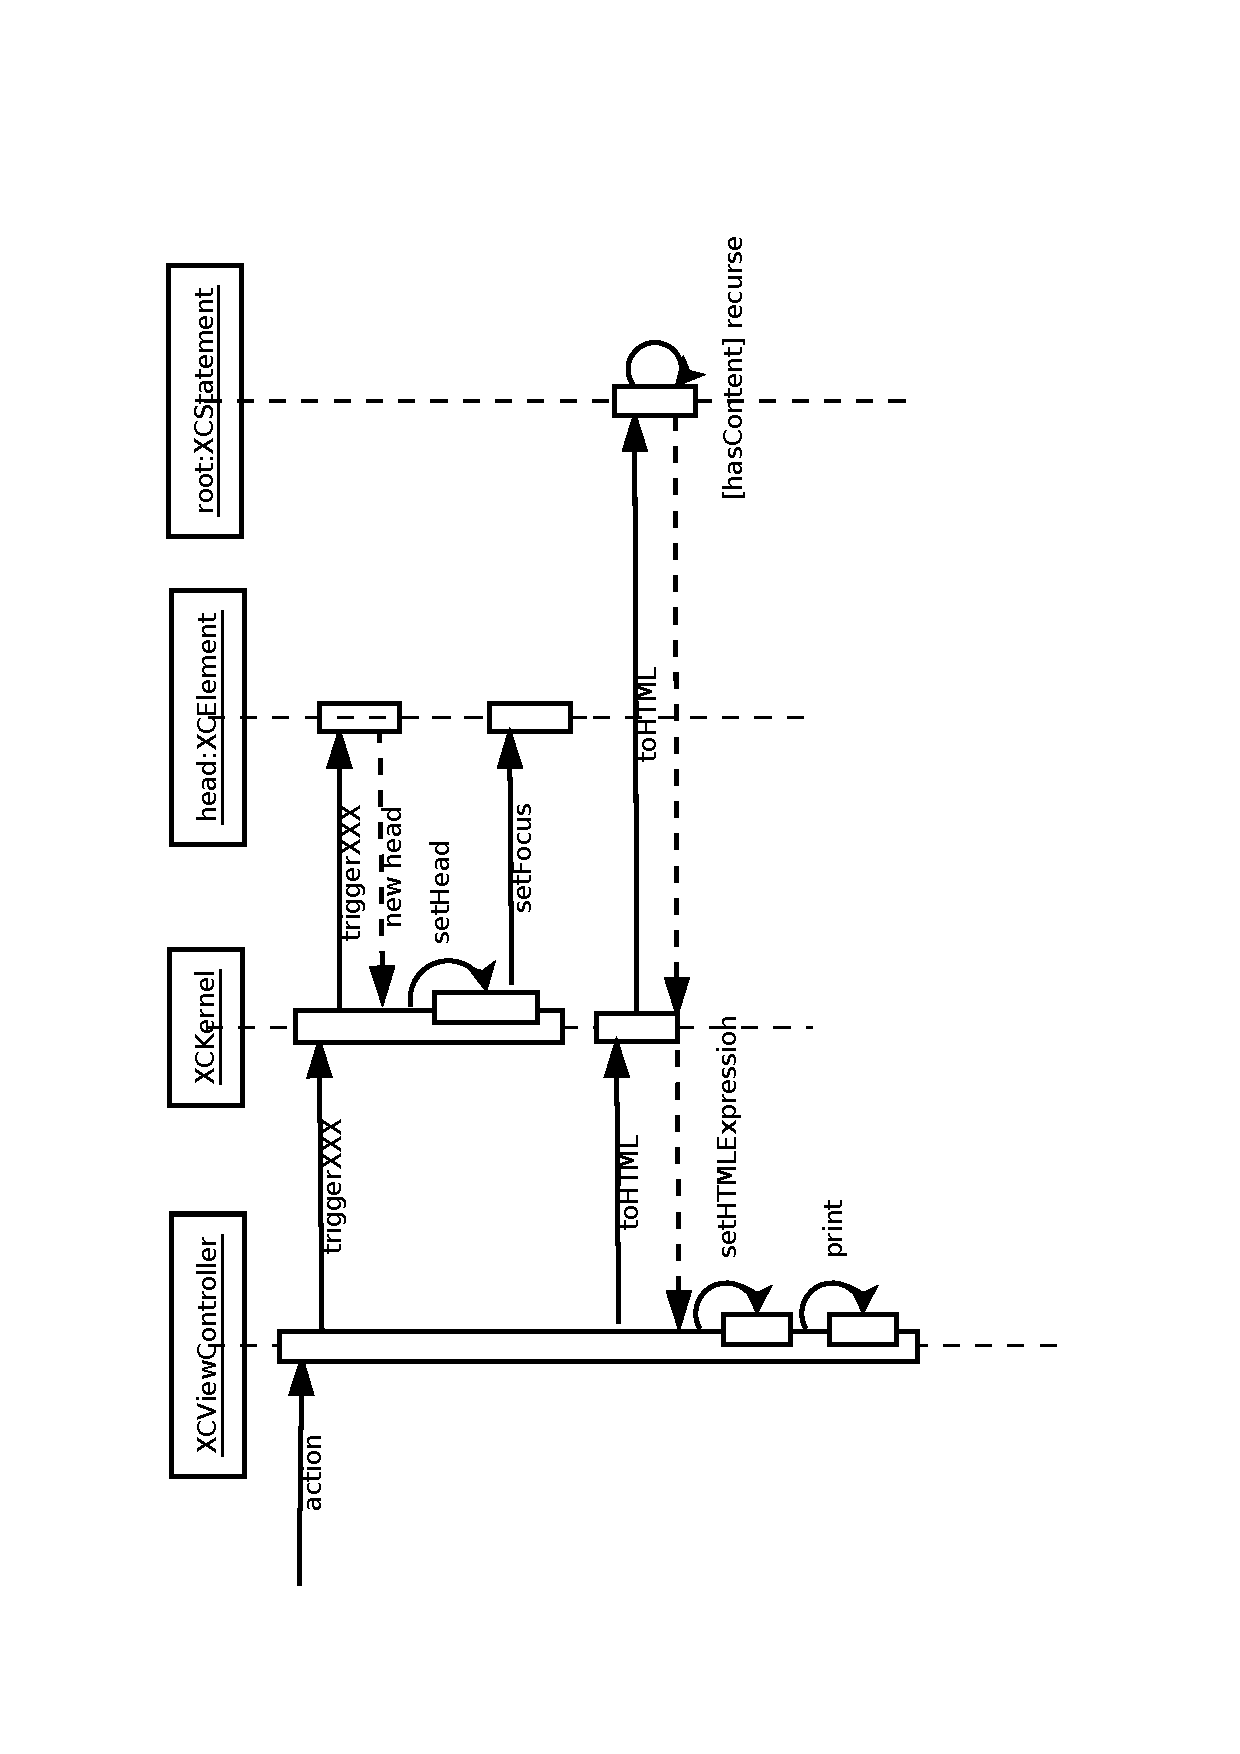
\includegraphics[angle=270, width=1\textwidth]{sq_trigger.pdf}
	\caption{Sequenzdiagramm: Trigger Allgemein}
\end{figure}
In diesem Kapitel soll der der allgemeine Programmablauf dargestellt werden.
Einzelne Klassen werden hier schon mal kurz angesprochen, aber erst im nächsten Kapitel eingehender behandelt.
\section{Eingabe von Symbolen}
Dieser Abschnitt zeigt den generellen Ablauf bei Eingaben durch den Benutzer. Anschließend wird noch ein ausgewähltes Beispiel vorgestellt werden.
\subsection{Allgemein}
Diagramm \ref{dia:sq:trigger} zeigt den allgemeinen Ablauf, wenn der Benutzer einen Button auf der View betätigt.
\begin{enumerate}
	\item Durch Betätigung eines Buttons wird im ViewController eine Action ausgelöst.
	\item Im VC wird eine entsprechende \code{trigger}-Nachricht an den Kernel (XCKernel-Klasse) geschickt.
		Triggernachrichten haben immer die Form:
		\begin{lstlisting}
			hasTriggers triggerXXX [ args ]
		\end{lstlisting}
		\begin{itemize}
			\item \code{hasTriggers} ist dabei der Rückgabewert, also ein Element welches wieder Trigger besitzt. Tatsächlich implementieren alle Elemente des Syntaxbaums sowie der Kernel das Protocol XCHasTriggers. 
			\item \code{triggerXXX} ist der Methodenname, wobei ``trigger'' immer als Präfix steht und ``XXX'' das eigentliche ``Zeichen'' ist, welches eingegeben werden soll.
			\item \code{[ args ]} bei manchen Triggermethoden müssen noch Argumente mitgegeben werden.
		\end{itemize}
	\item Der Kernel gibt den Triggeraufruf an das Headelement weiter. Head ist praktisch das Element im Syntaxbaum, auf dem der Focus bzw. der Cursor steht. Dieses wird dann im HTML-output hervorgehoben.
	\item Das Element entscheidet nun wie mit dem Triggeraufruf zu verfahren ist. 
		Dabei gibt es in der Regel folgende Möglichkeiten:
		\begin{enumerate}[I]
			\item Je nach Element und Kontext werden neue Elemente erzeugt und im Baum eingehängt, 
				wobei es vorkommen kann, dass sich das aufgerufene Objekt dabei selbst ersetzt. 
				Dabei wird auch meist eine neuer Platzhalter erzeugt, der zurückgegeben wird. 
			\item Das Element gibt den Aufruf an sein Elternelement im Baum weiter. 
			\item Im Zweifelsfall gibt sich das Element selbst zurück, ignoriert also den Knopfdruck des Benutzers.
		\end{enumerate}

	\item Der Kernel setzt nun den head neu, löscht den Focus (Bitflag) vom ehemaligen Head und setzt den Focus beim neuen Head
	\item Anschließend ruft der der ViewController die \code{toHTML}-Methode im Kernel auf, welcher diesen Aufruf an das Root-element des Baums weitergibt. Das HTML wird nun rekursiv erzeugt und nach Fertigstellung in ein Template eingesetzt und in einer UIWebView dargestellt.
\end{enumerate}

\subsection{Beispiel XCSpacer-triggerNum}
\begin{figure}[H]
	\centering
	\label{dia:sq:spacer}
	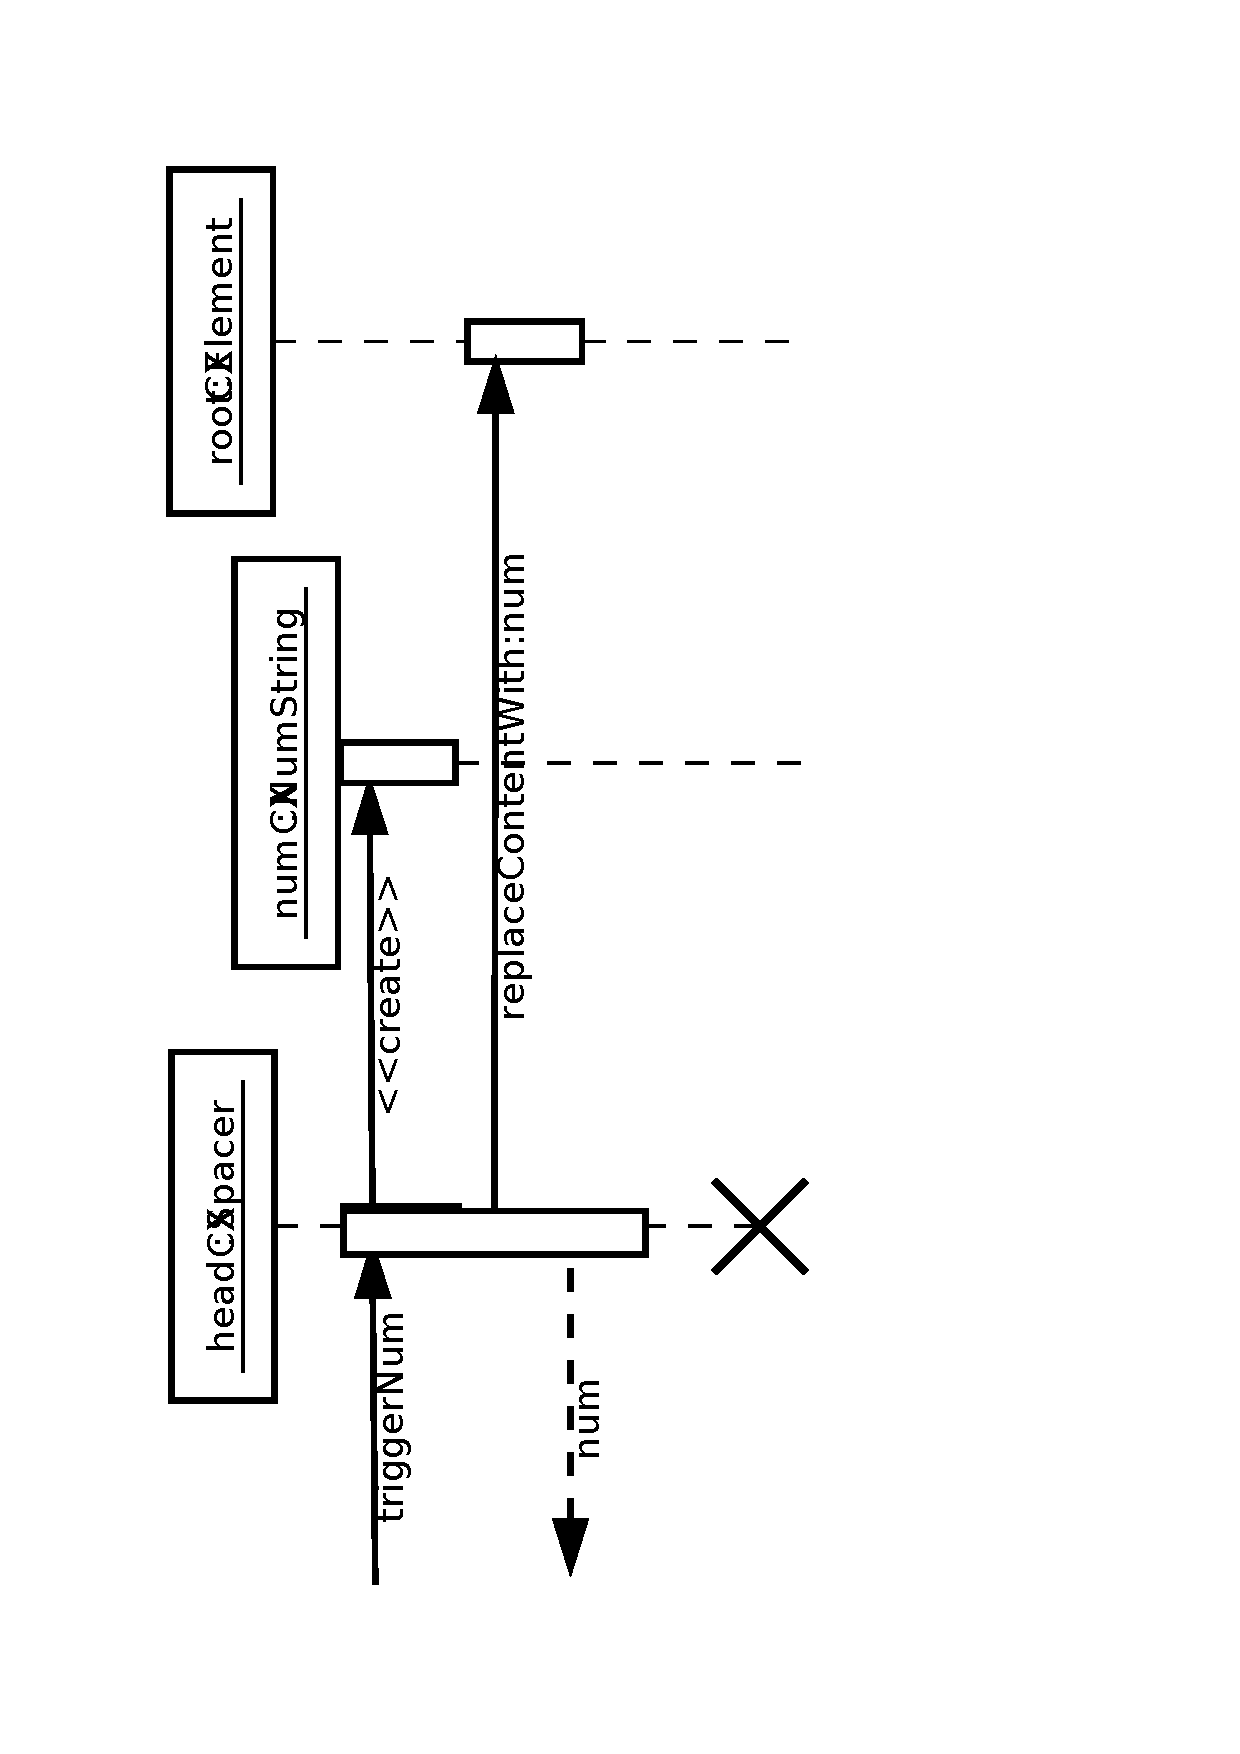
\includegraphics[angle=270, width=1\textwidth]{sq_spacer.pdf}
	\caption{Sequenzdiagrammfragment: triggerNum auf XCSpacer}
\end{figure}
Der Interne Ablauf im Baum bei einem Triggeraufruf soll nun anhand eines Beispiels gezeigt werden.
Das Diagrammfragment \ref{dia:sq:spacer} zeigt den Aufruf von {triggerNum} auf einem XCSpacer-objekt.

XCSpacer ist das Analogon zum Literal in der Grammatik und fungiert als Platzhalter für Zahlen, Funktionen, Konstanten, Variablen oder geschachtelte Ausdrücke. Der Spacer wird immer dann eingesetzt, wenn auf die Eingabe von Literale ``gewartet'' wird, also nach der Eingabe von Operatoren oder am Anfang, wenn ein leerer Ausdruck dasteht. 
\paragraph{Nun zum Beispiel:}
\begin{enumerate}
	\item die triggerNum-Methode von XCSpacer erzeugt eine neue \code{XCNumString}-Instanz.
		Dies ist ein Stringbuffer für Dezimalzahlen.
	\item XCSpacer ruft sein Elternelement auf und gibt ihm die Nachricht den aktuellen Inhalt (also sich selbst) mit der \code{XCNumString}-instanz zu ersetzen.
	\item zuletzt wird das neue XCNumString-objekt zurückgegeben und wie oben beschrieben weiterverfahren (Head neu gesetzt, HTML ausgegeben\ldots).
	\item Nachdem der Spacer weder im Kernel noch im Syntaxbaum referenziert ist, wird er zerstört.
\end{enumerate}
\subsection{Beispiel Operatoraufruf}
Hier noch ein kurzes Beispiel in Textform:
\begin{enumerate}
	\item Es wurde bereits folgendes eingegeben: '5+4*3', der Focus steht auf der '3'.
		In der \code{description}-Methodenschreibweise sieht der Ausdruck so Aus: \code{+(5, *(4, 3))}
		\footnote{Bei den Elementen handelt es sich entweder wie bei den Operatoren um Tupel 
			mit der Schreibweise \code{<Operator>(<Operand1>, Operand2)}, 
			Elemente mit einem Element als Inhalt (\code{<Name>(<Element>)}) oder um Terminalsymbol (-elemente).
		}
	\item Nun  wird '+' eingegeben.
		Es wird die Methode \code{triggerOperator} auf dem Element '3' aufgerufen. 
		Diese erkennt, dass das Elternelement ein Produkt ist und 
		gibt den Aufruf an dieses weiter.
		\begin{lstlisting}
			return [parent triggerOperator: op];
		\end{lstlisting}
	\item Da das Elternlement des Produktelements '4*3' eine Summe ist, 
		erzeugt dieses ein neues Summenelement mit sich selbst und einem Platzhalter als Parameter. Anschließend ersetzt es sich selbst im Elternknoten mit der neuen Summe. Der Ausdruck sieht nun wie folgt aus: \code{+(5, +(*(4, 3), _))}
	\item Zuletzt wird der Platzhalter als neues Head-Element zurückgegeben.
	\item Es wird nun noch die '2' gedrückt, welche den Platzhalter ersetzt.
	\item Die Ausgabe auf dem Bildschirm ist nun '5 + 4 * 3 + 2'
	\item Drückt man '=' wird der Ausdruck wie folgt ausgewertet: $((4 \cdot 3) + 2) + 5 = 19$ s.u.
\end{enumerate}


\section{Berechnung von Ausdrücken}
\begin{figure}[H]
	\centering
	\label{dia:sq:eval}
	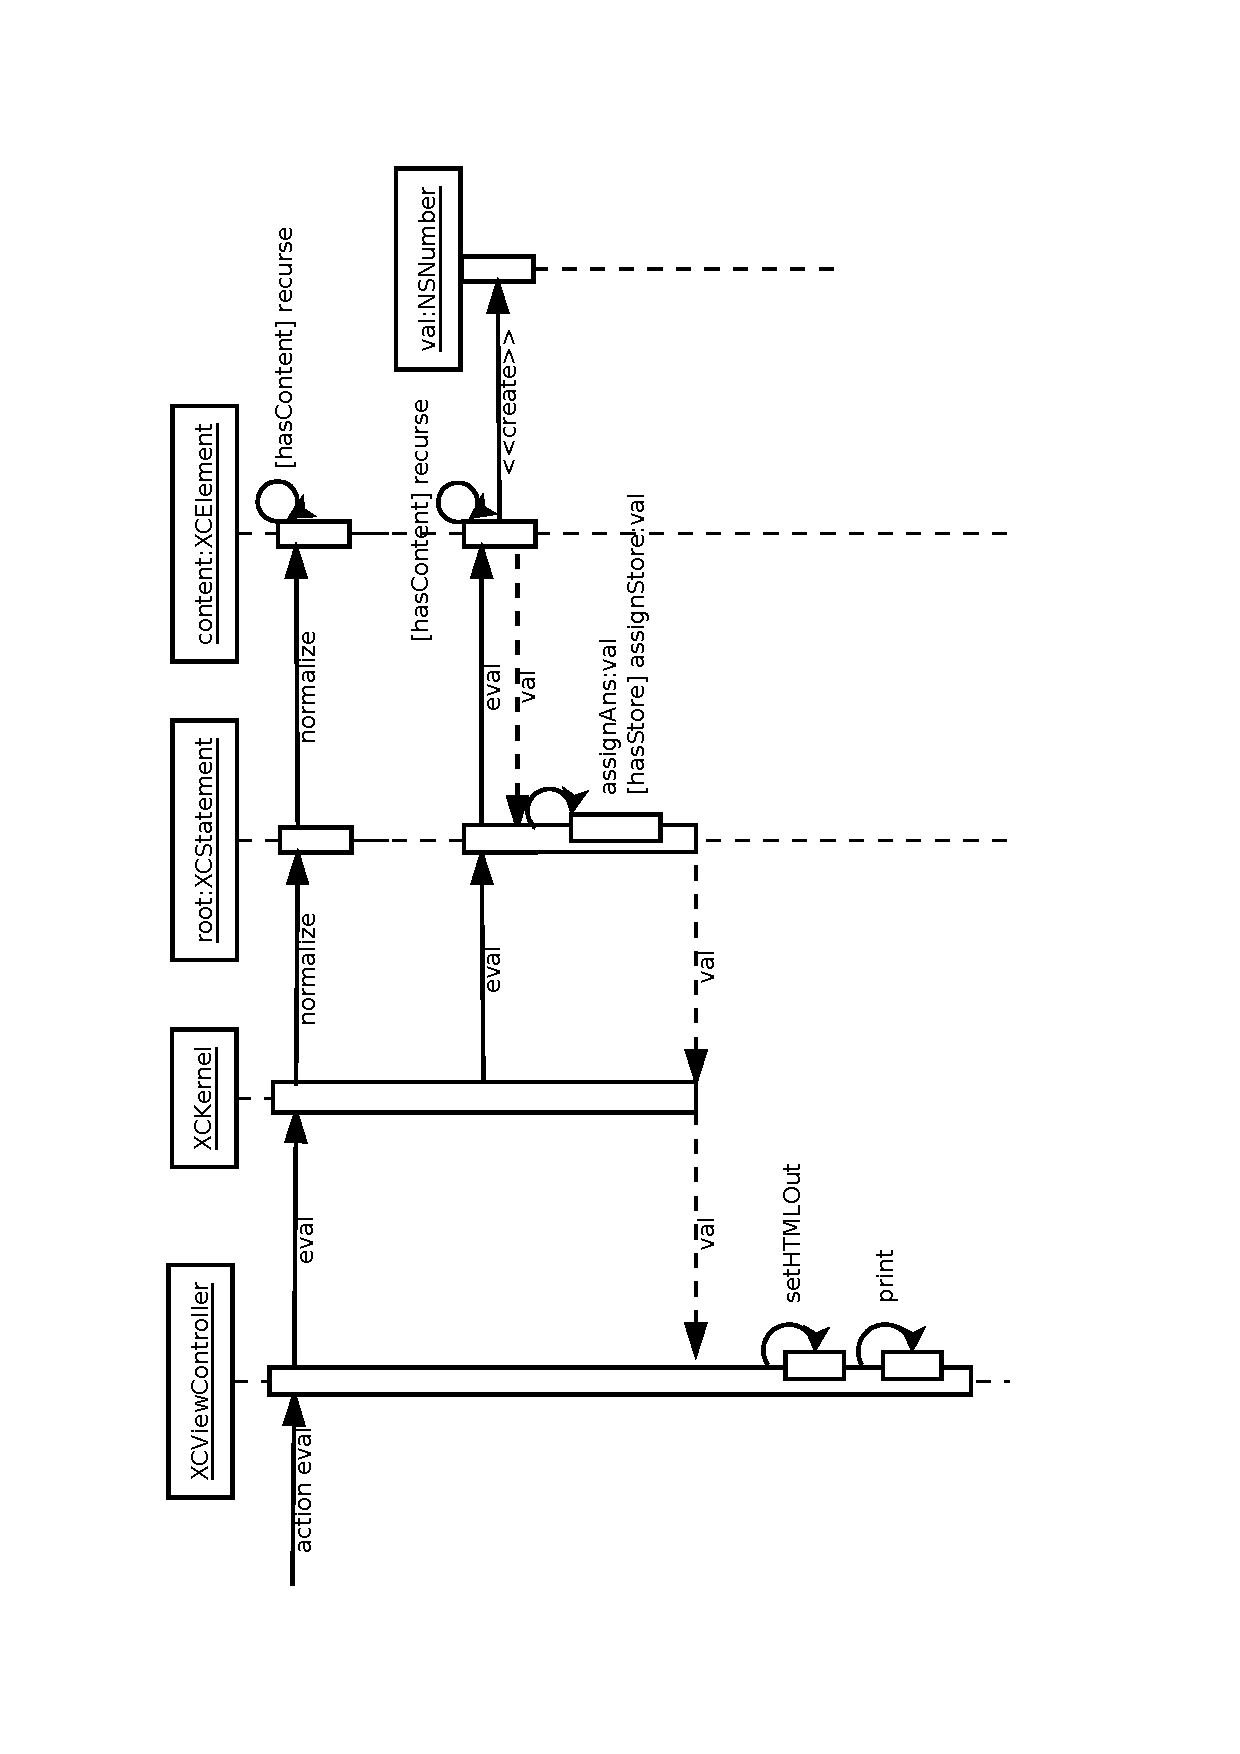
\includegraphics[angle=270, width=1\textwidth]{sq_eval.pdf}
	\caption{Sequenzdiagramm: eval}
\end{figure}
Es wird nun die Berechnung von Ausdrücken in allgemeiner Form beschrieben:
\begin{enumerate}
	\item Nach dem Drücken des ``=''-Buttons wird die \code{eval} am Kernel aufgerufen. 

	\item Diese leitet einen Normalisierung auf dem Syntaxbaum ein. Dabei werden z.B. Vorzeichen aufgelöst (z.B. $\frac 1 {-3} \implies -\frac1 3$).  
	\item Anschließend wird der Baum rekursiv evaluiert.
	Dabei wird Bottom-Up der Ausdruck ausgewertet (evtl. Fehlerflags gesetzt) und 
	die Zwischenergebnisse in Form von NSNumber objekten an den Aufrufer zurückgegeben.  
	\item im Root-Element des Baums (immer XCStatement) wird schließlich noch der Wert in der ANS-Variable gesetzt. Eine eventuell mit ``STO'' gesetzte Variable wird auch noch überschrieben.  
	\item Das zurückgegebene Ergebnis wird im ViewController in der WebView dargestellt.
\end{enumerate}

\chapter{Klassen}
In diesem Kapitel wird näher auf die wichtigsten Klassen und die Architektur eingegangen.
Das Programm ist aufgeteilt in den XCKernel-Bereich, welcher den inner Zustand des Taschenrechners verwaltet
und XCViewController-Bereich, in dem die View gesteuert wird. Der XCViewController benutzt dabei den Kernel.
\section{XCViewController}
\begin{figure}[H]
	\centering
	\label{dia:sq:eval}
	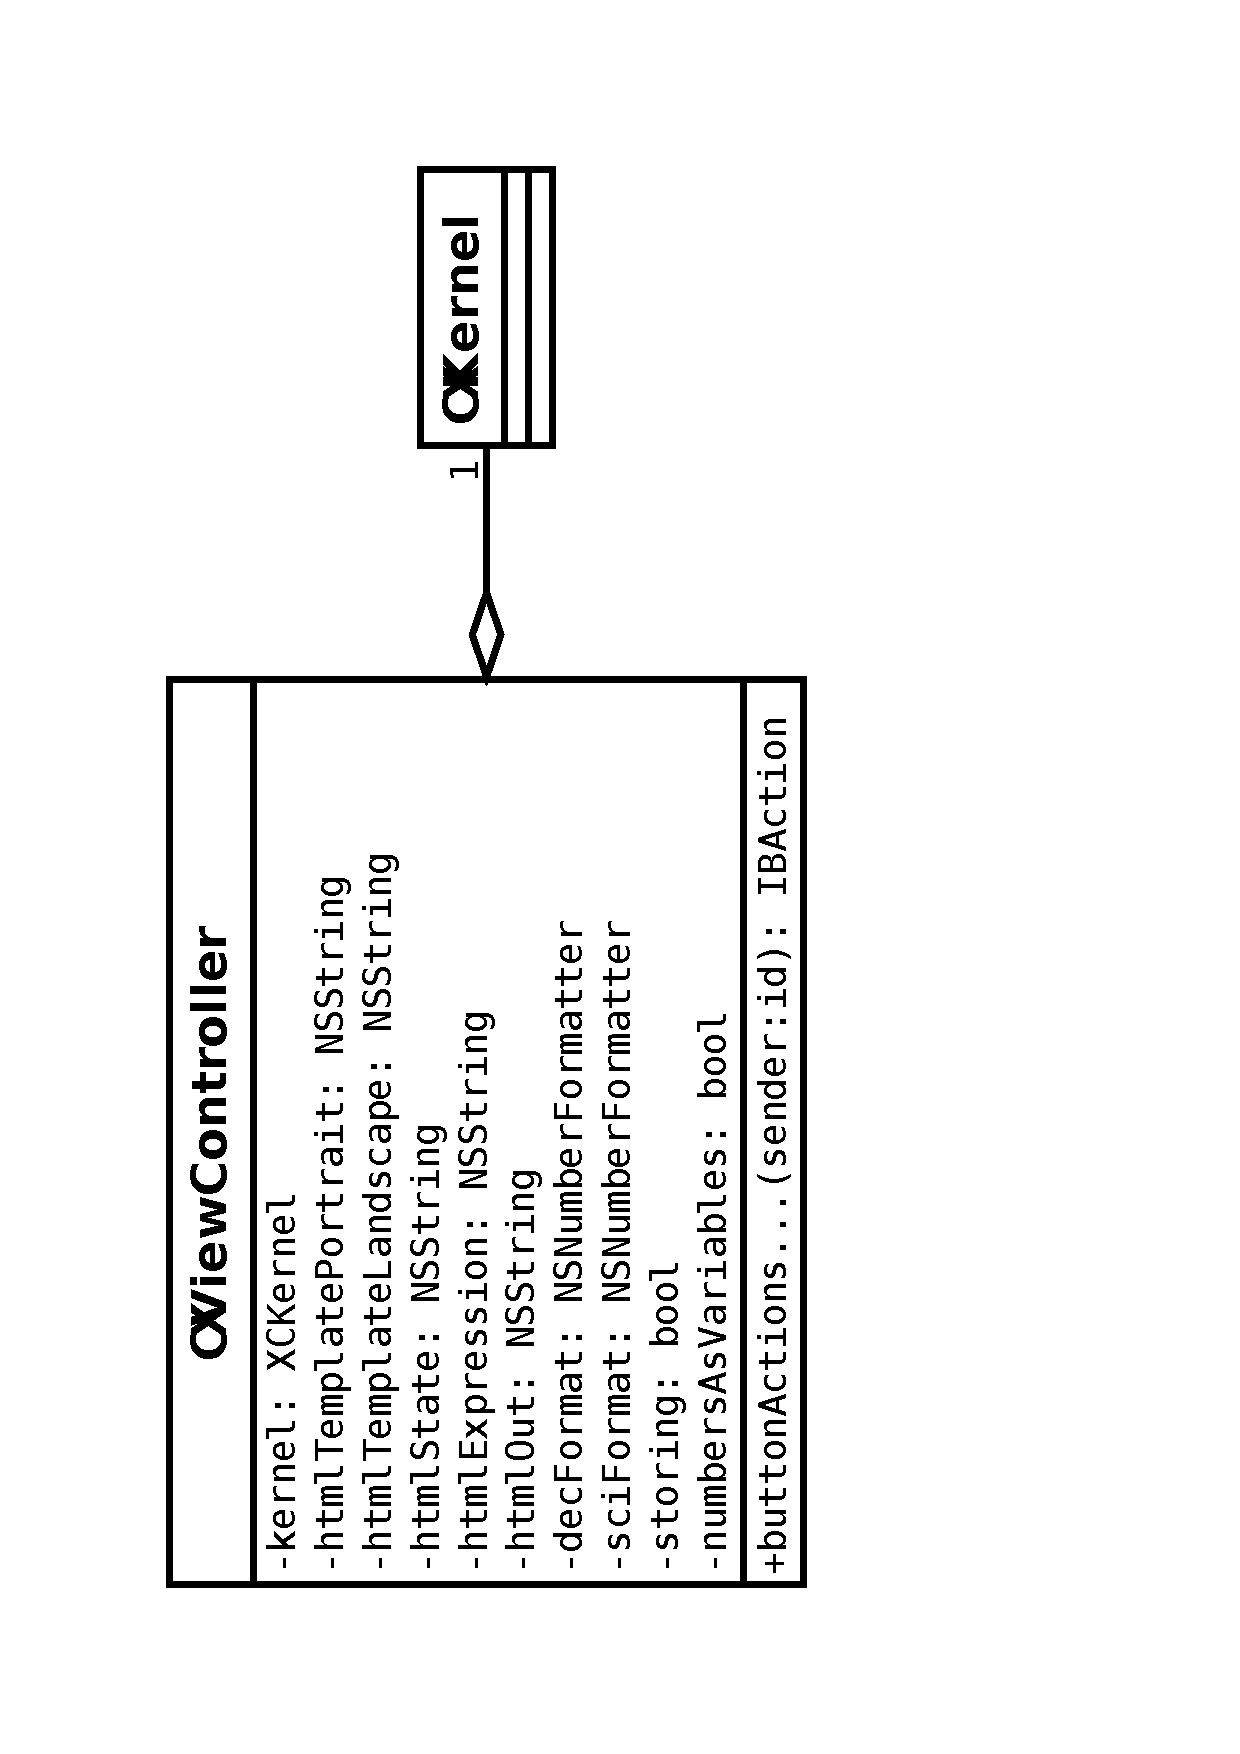
\includegraphics[angle=270, width=1\textwidth]{cl_vc.pdf}
	\caption{Klassendiagramm}
\end{figure}
Der ViewController verwaltet seinen Zustand den er zum Darstellen des Displays und zum Ansteuern der Trigger im Kernel benötigt.
Außerdem wird geregelt, wie die Tasten dargestellt werden sollen (z.B. Zahlen$\iff$ Variablen, DEG$\iff$RAD). Der Kernel (s.u.) übernimmt die eigentliche Aufgabe der Eingabe neuer Zeichen und der Berechnung.

\section{Kernel}
(siehe auch extra Klassendiagramm)
\subsection{Schnittstellen (Protocols)}
Viele Schnittstellen von häufig verwendeten Methoden(-gruppen) werden in folgenden Protocols zusammengefasst:
\begin{description}
	\item[XCHasHtmlOutput] Die Implementierung kann ihren Inhalt in (mathml)-HTML ausgeben. 
	\item[XCHasTriggers] Die Implementierung hat Trigger (siehe oben), kann also Eingabe durch den Benutzer verarbeiten.
	\item[XCEvaluable] Die Implementierung kann ihren Inhalt als NSNumber (berechnen und) zurückgeben.
\end{description}
\subsection{XCKernel}
Der Kernel verwaltet das Root-Element (XCStatement) des Syntaxtrees und das Head-Element, auf welchem der Focus steht. Außerdem enthält er einen Buffer (XCStatementBuffer), der die letzten Eingaben in einem Ringpuffer (XCCircBuf) abrufbar verwaltet.
\subsection{Hilfsklassen}
\begin{description}
	\item[NSNumber+XCNumber] Hierbei handelt es sich um eine Obj C Category, welche NSNumber um die unten benötigten Operatoren und einige Zustandsabfragen erweitert. 
		Außerdem wird eine interne Typ und Überlaufskontrolle durchgeführt. 
		Dabei werden eingegebene Integerwerte erhalten und im Fall von Überläufen in double konvertiert.
	Eine Erkennung von ganzzahligen double-Werten ist auch enthalten.
	\item[XCGlobal] Dies ist zum einen eine Art global.h, welche globale symbolische Konstanten enthält, aber auch eine Singleton-Klasse, welche globale Werte verwaltet (derzeit nur die Grad/Bogenmaß Winkeleinstellung)
\end{description}
\subsection{Syntax-Tree}
Die Oberklasse für alle Elemente des Syntaxbaums ist die Klasse XCElement.
Diese ist konform zu allen oben genannten Protokollen und NSCopying 
\footnote{Wird beim Wiederholen aus dem Statementbuffer benötigt, damit beim Ändern keine alten Ausdrücke überschrieben werden}. 
Für alle Methoden wird eine Standardimplementierung angeboten. 
Unterklassen müssen dann nur ihr eigenes Verhalten implementieren.


Desweiteren ist ein Bitflag-struct zur Speicherung des inneren Zustands nebst Hilfsmethoden enthalten, die von den Unterklassen zur Erstellung der HTMLs benötigt werden.


Außerdem ist ein parent-Element vorhanden. 
Mittels content-Methode und parent ist der Syntaxbaum aufwärts und abwärts navigierbar.

Eine Ableitung von XCElement ist der bereits besprochene XCSpacer.
Alle weiteren Unterklassen von XCElement werden nochmals in drei Kategorien eingeteilt:

\subsubsection{XCTupleElement}
Diese Elemente enthalten zwei weitere Kindelemente und werden derzeit ausschließlich zur Implementierung der Operatoren verwendet.
\footnote{
	In einer vorherigen Version waren diese als ``komplexe'' Elemente mit einem MutableArray vorhanden. Die Tupleversion hat sich aber letztendlich als einfacher erwiesen.
}

\paragraph{Unterklassen sind:} 
\begin{description}
	\item[XCSum] Die Summe. Negative Werte werden in XCNegate verpackt.
		Anders als in Grammatik wird der ``geklammerte Ausdruck'' aber extra behandelt: siehe XCExpression.
	\item[XCProduct] Das Produkt. Divisionen werden in Form von XCInvert dargestellt.
	\item[XCExponentiation] Der Exponetialoperator
\end{description}

\subsubsection{XCSimpleElement}
Die simplen Elemente enthalten immer nur ein weiteres Element.
\paragraph{Unterklassen sind:} 
\begin{description}
	\item[XCStatement]
		Analog zur Grammatik bildet das Statement immer das Root-Element eines Syntaxbaums. Es enthält einen Ausdruck, der berechnet werden kann sowie optional eine explizit zugewiesene Variable, welcher nach der Berechnung das Ergebnis eingesetzt wird. Implizit wird immer das Ergebnis der ANS-Variable zugewiesen. 
	\item[XCFunction] Die Funktion besteht aus einem Name und einem Ausdruck, dessen Ergebnis in die Funktion eingesetzt wird. Die Klasse verwaltet ein Dictionary von XCFuncAlg-instanzen (XCTrigoFuncAlg für Winkelfunktionen). Diese enthalten die eigentliche Funktion als Functionpointer.
		XCSqrt ist eine Spezialisierung von XCFunction, es wird lediglich die toHTML-Methode für die Wurzeldarstellung überschrieben.
	\item[XCValModifier] Diese Elemente neutralisieren sich selbst und ein hinzugefügtes Element, falls dieses vom gleichen Typ ist.
		Beispiel: aus -(-2) wird 2.
		Weitere Unterklassen sind:
		\begin{description}
			\item[XCInvert]
				Invertiert einen Wert. Wird unter anderem von XCProduct verwendet, da diese Klasse nur multiplizieren kann.
			\item[XCNegate] Der enthaltene Wert wird negiert. Analog zu XCInvert: von XCSum zur 
				Darstellung von Minus benutzt.
			\item[XCExpression] Kapselt einen weiteren Ausdruck.
		\end{description}
\end{description}
\subsubsection{XCTerminalElement}
Wie der Name schon andeutet handelt es sich dabei um die Implementierung der Terminalsymboleaus der Grammatik. Naturgemäß enthalten diese keine weiteren Syntaxelemente und bilden die Blätter des Syntaxbaums.

\paragraph{Unterklassen sind:} 
\begin{description}
	\item[XCIdentifier] enthält ein XCStorage-objekt, also eine Variable (XCVariable) oder eine Konstante (XCConstant).
	\item[XCNumString] Diese Klasse hat lediglich einen String-Buffer mit dem Dezimalzahlen erstellt werden können (also Digits und Komma). Die Klasse ist hinreichend intelligent um falsche Eingaben, wie mehrfaches Komma abzufangen.
		Beim Aufruf von eval wird der Buffer geparst und in ein NSNumber umgewandelt.
\end{description}

\chapter{Tests}
Grundlegende Funktionalitäten wurden mit Unittests erfasst, dabei wurde folgendes getestet:
\begin{itemize}
	\item korrekte Berechnung duch die NSNumber-Category
	\item richtige Auswertung von Ausdrücken anhand der einzelnen Elemente.
	\item XCKernelTest: Hier wird mittels der trigger-Methoden mehrere Eingaben von Ausdrücken getestet.
	\item Auswertung nach der Normalisierung.
	\item Grundlegende Klassen wie der XCStatementBuffer
\end{itemize}
Das dynamische Verhalten wurde ``am lebenden Objekt'' immer wieder getestet:
\begin{itemize}
	\item Ausgabe von HTML
	\item Verhalten bei der Navigation und beim Löschen
	\item Aufrufreihenfolge bei Operatoren.
	\item Verhalten des XCViewControllers
\end{itemize}
